\chapter{行为生态学}\label{ch:b3:behavioural-ecology}

一只猫鼬站在白蚁丘上，群中其余个体正在挖掘食物，
一旦出现鹰，它便鸣叫示警，其他个体纷纷奔向
洞穴。哨兵已一小时没有进食，
却使自己成了沙漠中最显眼的动物。为什么？一只孔雀拖着
一条尾羽，耗去它五分之一的能量预算，还拖慢了它
逃离老虎的速度。一只从田野归来的蜜蜂，在竖直方向的
巢脾上跳舞，其舞蹈与竖直方向的夹角，即为
食物与太阳的夹角。一只大山雀在一片树丛中捕食毛毛虫，
在仍有毛毛虫可找的时候便离开这片树丛。
这些动物没有一个读过本章，但每一个的行为都仿佛
已解出了一道最优化问题、一场博弈，或一道亲缘关系核算题。行为生态学
是把行为当作一组演化而来的解决方案来研究的学科：
一种行为有何用处（就其所传播的基因而言），以及
其代价与收益必须是怎样的，自然选择才会产生它。
它的工具与经济学家所用的相同：最优化、\omterm{prop:b3:behavioural-ecology:hawk-dove}{博弈论}、
亲缘关系核算；而其检验则在野外进行。

\section{四个问题与本能的机制}

\begin{definition}[廷伯根的四个问题]\label{def:b3:behavioural-ecology:tinbergen}
\index{廷伯根的四个问题}\index{固定动作模式}\index{信号刺激}\index{印随}\index{关键期}
廷伯根（1963）指出，对任何一种行为的完整说明必须回答
四个问题：其\emph{机制}（何种刺激与神经结构
产生它），其\emph{发育}（它如何在个体中形成，
由基因与经验共同决定），其\emph{功能}（它如何有助于
生存与繁殖），以及其\emph{演化历史}（它如何
由祖先行为演化而来）。提出这些问题的动物行为学家
已建立了前两个问题。许多行为是\emph{固定动作
模式}：由简单的\emph{信号
刺激}触发、一经开始便进行到底的刻板序列——一只灰雁用喙把滚出巢外的卵
滚回巢中，即使卵在中途被拿走，它仍会完成这一动作；
一只银鸥雏鸟会啄任何形似喙的物体上的红色斑点，
并且更多地啄带三道红色条纹的木棍，而非真正的
银鸥头部；一条雄性刺鱼会攻击其腹部为红色的任何东西，
包括透过车窗看见的驶过的邮车。另一些行为则在
一个时间窗内习得：\emph{印随}，即
小鹅在出生后第一天跟随并此后视为父母的
任何移动之物——一只鹅、洛伦茨或一个纸箱——这一过程迅速、
不可逆，且限于\emph{关键期}之内；鸟类的鸣唱学习
即本科二年级分册中的例子，其模式与此相同。二分法
把行为分为先天与习得是错误的：一种行为具有一套遗传程序，
规定学什么、何时学、向谁学，而这一程序
正是演化的对象。
\end{definition}

\begin{proof}[证据]
廷伯根的野外实验确立了这一方法。掘穴蜂
（\emph{Philanthus}）飞回藏在沙中的巢穴；他在蜂离开时
将其一个洞口周围的一圈松果移动了位置，
蜂便在移动后的圆环中心搜寻——它已记住了
这些地标。红嘴鸥在孵化后将蛋壳移出巢外。他
将卵摆放在涂色的蛋壳、天然蛋壳及
其他物体旁边，并统计乌鸦拿走了哪些：
蛋壳内表面白色的部分吸引了捕食者，而看似
整洁的移除行为实为伪装。银鸥雏鸟的实验对\omterm{def:b3:behavioural-ecology:tinbergen}{信号刺激}做了
定量研究：提供纸板做的头部模型，每次只改变
一个特征。洛伦茨\omterm{def:b3:behavioural-ecology:tinbergen}{印随}的鹅终生跟随他；鸭子
在第一天便对移动的纸箱形成\omterm{def:b3:behavioural-ecology:tinbergen}{印随}，此后
即便让它们去跟随鸭子，也无法做到。
\end{proof}

\begin{omfigure}
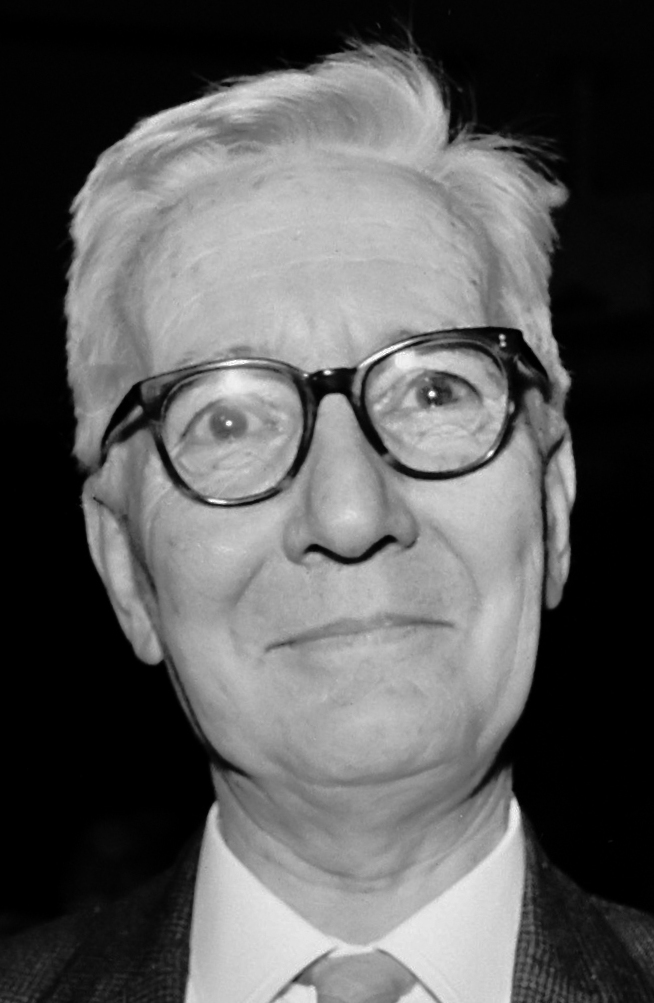
\includegraphics[width=0.36\linewidth]{images/book5/tinbergen.jpg}\hspace{0.04\linewidth}
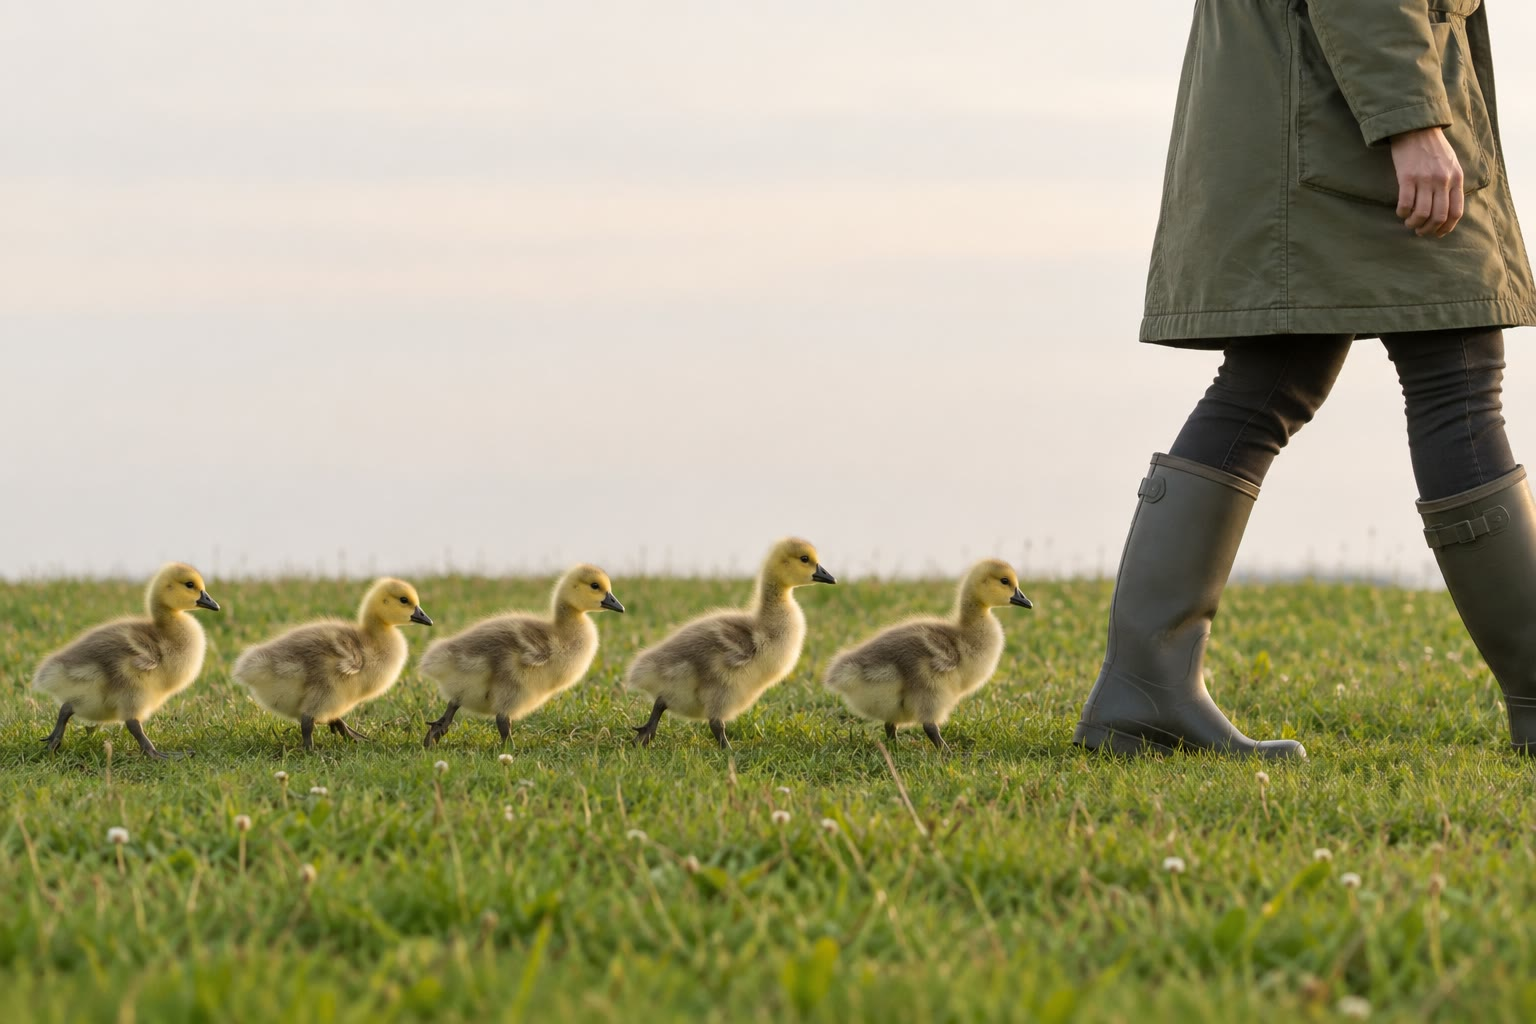
\includegraphics[width=0.52\linewidth]{images/book5/ai/b5-26-goose-imprinting.jpg}

{\small 左：尼可·廷伯根（1907--1988），他将行为的问题带入野外，使之
实验化（
照片：Rob Mieremet, Anefo, 1973, CC0）。右：小鹅在孵化后一天内跟随所见的第一个大型移动物体，
此后便再也无法被说服
改变。}
\end{omfigure}

\section{决策：最优觅食}

\begin{theorem}[边际值定理]\label{thm:b3:behavioural-ecology:mvt}
\index{最优觅食}\index{边际值定理}\index{斑块停留时间}\index{通货}
觅食者访问若干食物斑块，相邻斑块之间相隔旅行时间 $\tau$。在一个
斑块中，获得的能量为 $g(t)$，经过时间 $t$ 后，$g$ 递增且
凹（斑块逐渐耗竭）。若它在经过时间 $t$ 后离开每个斑块，
其长期平均获能速率为 $R(t) = g(t)/(\tau + t)$，
使之最大的停留时间 $t^{*}$ 满足
\[
g'(t^{*}) = \frac{g(t^{*})}{\tau + t^{*}} = R(t^{*}) :
\]
当斑块中的瞬时获能速率降至
包括旅行在内的整个生境的平均速率时离开（查诺夫，
1976）。由此可得：旅行时间越长，停留越久，
每个斑块被耗竭得越彻底；在更丰富的生境中
（$R$ 更高），每个斑块被更早离开、耗竭程度更低；所有
斑块都以相同的边际速率离开，无论其品质如何，因此
贫瘠的斑块几乎立即被放弃，而丰富的斑块则
只有在其被耗竭至生境平均水平时才离开。对于 $g(t) = A(1 -
\mathrm{e}^{-t/T_{0}})$，此时条件变为 $(\tau + t^{*})/T_{0} =
\mathrm{e}^{t^{*}/T_{0}} - 1$，需数值求解：当 $\tau = T_{0}$ 时，
$t^{*} \approx 1.15\,T_{0}$；当 $\tau = 4T_{0}$ 时，$t^{*} \approx
2.0\,T_{0}$。
\end{theorem}
\begin{proof}
$R(t) = g(t)/(\tau + t)$; $R'(t) = [g'(t)(\tau + t) - g(t)]/(\tau +
t)^{2} = 0$ 得 $g'(t^{*}) = g(t^{*})/(\tau + t^{*})$。从几何上看：
以 $g$ 对 $t$ 作图，原点取在 $-\tau$ 处；$R(t)$ 即为
从 $(-\tau, 0)$ 到 $(t, g(t))$ 的直线的斜率，当该直线
与曲线相切时最大——这即为上述条件。$\tau$ 增大
使原点左移，切点右移；更丰富的生境使切线变陡，
并使切点左移。对于指数函数，$g' = (A/T_{0})
\mathrm{e}^{-t/T_{0}}$ 及 $g/(\tau + t) = A(1 - \mathrm{e}^{-t/T_{0}})/
(\tau + t)$；令二者相等并整理，即得所述方程，
代入 $t^{*} = 1.15T_{0}$ 及 $\tau = T_{0}$：左边为 $2.15$，右边
$\mathrm{e}^{1.15} - 1 = 2.16$。
\end{proof}

\begin{omfigure}
\begin{tikzpicture}
\begin{axis}[
  width=0.68\linewidth, height=5.8cm,
  axis x line=middle, axis y line=left,
  xmin=-4.5, xmax=5, ymin=0, ymax=1.15,
  xlabel={时间（单位为 $T_{0}$）}, ylabel={斑块中获得的能量},
  xlabel style={font=\small, at={(axis description cs:0.95,0.0)}, anchor=north}, ylabel style={font=\small},
  tick label style={font=\small}, xtick={-4,-1,0,1.15,2}, xticklabels={$-4T_0$,$-T_0$,0,$1.15$,$2.0$}, ytick={0.5,1}, yticklabels={$0.5A$,$A$},
  clip=false,
]
\addplot[very thick, omDef, domain=0:5, samples=80] {1-exp(-x)};
\draw[thick, omThm] (axis cs:-1,0) -- (axis cs:1.55,1.13);
\draw[thick, omMeth!70!black] (axis cs:-4,0) -- (axis cs:3.5,1.081);
\fill[omThm] (axis cs:1.15,0.6834) circle (2pt); \fill[omMeth!70!black] (axis cs:2,0.8647) circle (2pt);
\draw[dashed, gray] (axis cs:1.15,0) -- (axis cs:1.15,0.6834); \draw[dashed, gray] (axis cs:2,0) -- (axis cs:2,0.8647);
\node[font=\scriptsize, omThm, anchor=north west, align=left] at (axis cs:-4.4,1.1) {短途旅行，$\tau = T_{0}$：\\在 $t^{*} = 1.15\,T_{0}$ 时离开，\\斑块已消耗\qty{68}{\%}};
\node[font=\scriptsize, omMeth!70!black, anchor=north west, align=left] at (axis cs:2.4,0.62) {长途旅行，$\tau = 4T_{0}$：\\在 $t^{*} = 2.0\,T_{0}$ 时离开，\\\qty{86}{\%}已消耗};
\node[font=\scriptsize, omDef, anchor=north west] at (axis cs:3.0,0.86) {$g(t) = A(1 - \mathrm{e}^{-t/T_{0}})$};
\node[font=\scriptsize, gray, anchor=south] at (axis cs:-2.5,0.02) {行程};
\end{axis}
\end{tikzpicture}

{\small 边际值定理示意图。随斑块被消耗，收益曲线逐渐变平；
从行程起点到曲线上某点的连线，其斜率等于
总体获取速率；最佳离开时刻
即为该连线与曲线相切之处。行程越长，原点左移，
切点右移。}
\end{omfigure}

\begin{proof}[证据]
考伊（1977）让大山雀在鸟舍中寻找藏于锯末杯中的黄粉虫，
并通过安装去除时间较长或较短的杯盖来调控杯间的行程时间；
鸟类在行程较慢时于每个杯中停留更久，
与定理的预测相符，
且略微超出预测，超出的方向
正是考虑行程能量消耗所能解释的。椋鸟衔运大蚊幼虫
回巢喂养雏鸟（卡切尼克，1984）时，从更远处的投食点
携带量更大，这同样符合负荷曲线速率最大化解的要求。
两项检验都不能证明鸟类会计算切线；
它们都表明，自然选择产生的是一些经验法则，
其结果接近最优。
\end{proof}

\section{竞争：博弈论}

\begin{proposition}[鹰鸽博弈与演化稳定策略]\label{prop:b3:behavioural-ecology:hawk-dove}
\index{博弈论}\index{鹰鸽博弈}\index{演化稳定策略}\index{频率依赖选择}
当最佳行为取决于他人的行为时，就不存在最优解，
只存在一场\emph{博弈}。两个动物争夺价值为 $V$ 的资源；一方
\emph{鹰}战斗直至受伤（代价为 $C$）或取胜，\emph{鸽}
受到攻击时展示并退让。平均收益如下：
\[
\begin{array}{c|cc}
 & \text{对鹰} & \text{对鸽}\\ \hline
\text{鹰} & (V - C)/2 & V\\
\text{鸽} & 0 & V/2
\end{array}
\]
一个\emph{\omterm{prop:b3:behavioural-ecology:hawk-dove}{演化稳定策略}}（梅纳德·史密斯与普莱斯，1973）
是这样一种策略：一旦成为群体中的常见策略，便不会被任何稀有的替代策略入侵。
若 $V > C$，则鹰即为 ESS：即使面对好斗者，战斗也有利可图。若 $V
< C$，两种纯策略都不稳定——全为鸽的种群会被
每场争斗都获胜的鹰入侵，全为鹰的种群会被
避免受伤的鸽入侵——ESS 则是以
概率采取鹰策略，其值为
\[
p^{*} = \frac{V}{C},
\]
或等价地，群体中该比例的个体为鹰。在
ESS 处两种策略收益相同，各自平均为 $V(1 -
V/C)/2$，低于全为鸽的种群所能分享的 $V/2$：争斗使
每个人都付出代价，任何人单独行动都无法获益更多。选择
在此是\emph{频率依赖的}：策略的适合度随其变得常见而下降，
这正是动物争斗多为展示、偶尔才演变为战争的原因，
也是这种混合状态得以持续的原因。
\end{proposition}
\begin{proof}
设比例为 $p$ 的个体采取鹰策略。鹰的期望收益为 $W_{H} = p(V
- C)/2 + (1 - p)V$；鸽的期望收益为 $W_{D} = (1 - p)V/2$。$W_{H} - W_{D} =
p(V - C)/2 + (1 - p)V/2 = [V - pC]/2$，当 $p < V/C$ 时为正，
比例较大时为负：鹰在稀少时扩散，在常见时被淘汰，且
频率稳定于 $W_{H} = W_{D}$ 处，即 $p^{*} = V/C$。其稳定性
由符号变化可知，对 $p$ 的扰动若高于
$p^{*}$，则有利于鸽并被纠正，低于其则有利于鹰。若 $V
\ge C$，则对所有 $p \le 1$ 差值均为正，鹰将固定。
在 $p^{*}$ 处的共同收益为：$W_{D} = (1 - V/C)V/2$。
\end{proof}

\begin{omfigure}
\begin{tikzpicture}
\begin{axis}[
  width=0.6\linewidth, height=5.4cm,
  axis x line=bottom, axis y line=left,
  xmin=0, xmax=1, ymin=-1, ymax=4.2,
  xlabel={鹰的比例 $p$}, ylabel={期望收益},
  xlabel style={font=\small, at={(axis description cs:0.5,-0.12)}, anchor=north}, ylabel style={font=\small},
  tick label style={font=\small}, xtick={0,0.5,1}, xticklabels={0,$p^{*} = V/C$,1}, ytick={0,1,2,4},
  clip=false,
]
\addplot[very thick, omThm, domain=0:1, samples=2] {x*(4-8)/2 + (1-x)*4};
\addplot[very thick, omDef, domain=0:1, samples=2] {(1-x)*4/2};
\draw[dashed, gray] (axis cs:0.5,-1) -- (axis cs:0.5,1);
\fill[black] (axis cs:0.5,1) circle (2pt);
\node[font=\scriptsize, omThm, anchor=north west] at (axis cs:0.5,3.9) {鹰：$p(V - C)/2 + (1 - p)V$};
\node[font=\scriptsize, omDef, anchor=south west] at (axis cs:0.62,0.9) {鸽：$(1 - p)V/2$};
\node[font=\scriptsize, anchor=west, align=left] at (axis cs:0.55,2.6) {$V = 4$，$C = 8$：\\ESS 位于 $p^{*} = 0.5$，\\收益 $V(1 - V/C)/2 = 1$};
\draw[->, thick, omThm] (axis cs:0.1,-0.5) -- (axis cs:0.4,-0.5); \draw[->, thick, omDef] (axis cs:0.9,-0.5) -- (axis cs:0.6,-0.5);
\node[font=\tiny, anchor=north] at (axis cs:0.25,-0.55) {鹰扩散}; \node[font=\tiny, anchor=north] at (axis cs:0.75,-0.55) {鸽扩散};
\end{axis}
\end{tikzpicture}

{\small \omterm{prop:b3:behavioural-ecology:hawk-dove}{鹰鸽博弈}。收益线相交之处，两种
策略收益相等，两者都无法扩散；在交点两侧，
选择会把频率推回。该混合状态稳定，并使所有个体付出代价，
这正是动物争斗的典型情形。}
\end{omfigure}

\begin{example}[野外博弈]\label{ex:b3:behavioural-ecology:games}
雄性斑林蝶争夺林地上的光斑：
占有者几乎总能在一次短暂的螺旋飞行中获胜，当两只
雄蝶被诱使各自都以为自己是占有者时，争斗
持续时间长十倍——一种约定（“占有者获胜”），它使争斗
得以低成本解决，它本身即为进化稳定策略，条件是争斗代价高昂，
而资源价值不大。雄性粪蝇守在牛粪饼上等候
雌蝇，并在到达率降至新鲜牛粪饼所能提供的水平时离开——
这又是边际值定理，只是在这一博弈中，斑块的价值
取决于其上有多少竞争者。榕小蜂、侧斑蜥，其雄性
有三种类型，彼此循环相克，如同石头–剪刀–布，
以及鲑鱼和蓝鳃太阳鱼中的“潜行”雄鱼，它们通过悄悄溜过
无法与之争斗的占有领地的雄鱼而使卵受精，
这些皆为混合状态，各策略在该频率下
收益相等。消耗战——两只动物相互炫耀，直至一方放弃，
其进化稳定策略是坚持一段由指数分布抽取的随机时间——
它描述了许多物种的对峙争斗，
并正确地预言：败者的坚持
不会泄露它原本还能坚持多久的信息。
\end{example}

\section{亲缘：哈密顿法则}

\begin{theorem}[哈密顿法则]\label{thm:b3:behavioural-ecology:hamilton}
\index{哈密顿法则}\index{亲缘选择}\index{亲缘系数}\index{广义适合度}\index{利他行为}\index{单双倍性}
若某等位基因使其携带者实施某种行为，令其损失 $c$ 个
后代，同时使一名亲属额外获得 $b$ 个后代，则该等位基因会扩散，条件是
\[
r\,b > c ,
\]
其中 $r$ 为\emph{\omterm{thm:b3:behavioural-ecology:hamilton}{亲缘系数}}：受体中某一基因
是行为者中同一基因经由祖先遗传而来的拷贝的概率——
亲代与子代或全同胞为 $1/2$，
半同胞、孙辈、侄甥辈为 $1/4$，一级表亲为 $1/8$。
该等位基因所最大化的量是其携带者的
\emph{\omterm{thm:b3:behavioural-ecology:hamilton}{广义适合度}}：其自身的繁殖，加上其对亲属繁殖的影响，
各项以 $r$ 加权。\emph{\omterm{thm:b3:behavioural-ecology:hamilton}{利他行为}}——降低行为者自身的繁殖、
提高他人繁殖的行为，
因而朝亲缘方向演化，程度与\omterm{thm:b3:behavioural-ecology:hamilton}{亲缘系数}成正比。该法则预测
其应出现之处：雌性地松鼠的报警鸣叫，
它们与姐妹和女儿共居，而非
雄性（它们会迁散）；猫鼬放哨，其群体即为一个家庭；
在鸟类的巢中，助巢个体协助双亲
抚育兄弟姐妹，当领地已满时。在
\emph{\omterm{thm:b3:behavioural-ecology:hamilton}{单双倍性}}的膜翅目昆虫中——雄虫由未受精卵发育而来，
只有一套染色体，雌虫则有两套——全同胞姐妹共享
四分之三的基因（$r = 3/4$），多于母亲与其女儿所共享的
（$1/2$）。哈密顿据此提出，
蚂蚁、蜜蜂和黄蜂中的不育工蜂品级在此出现了十一次，
而在其他类群中几乎从未出现。
\end{theorem}
\begin{proof}
考虑该等位基因的拷贝。行为者实施该行为时，
其自身的拷贝在期望传递中损失 $c$；
受体携带该等位基因的概率比群体平均值高出 $r$，
因此受体所得收益 $b$ 使该等位基因的传递
平均增加 $rb$。当 $rb - c > 0$ 时，该等位基因频率上升
（哈密顿，1964；一般推导基于个体基因型与其适合度之间的协方差，
即普赖斯方程，
在本阶段不加证明地承认）。\omterm{thm:b3:behavioural-ecology:hamilton}{亲缘系数}：亲代将每个基因以
$1/2$ 的概率传给子代；两个全同胞各自从同一亲代获得某一基因的
同一亲代的概率为 $1/2$，且二者为同一拷贝的概率为
$1/2$，亲代有两个，故 $r = 2\times\tfrac{1}{2}
\times\tfrac{1}{2} = \tfrac{1}{2}$。\omterm{thm:b3:behavioural-ecology:hamilton}{单双倍性}的姐妹：
她们从单倍体父亲处获得相同基因（概率为 $1$）；
从母亲处获得相同拷贝的概率为 $1/2$；
对两个亲代取平均，得 $r = (1 + 1/2)/2 = 3/4$。
\end{proof}

\begin{omfigure}
\begin{tikzpicture}[every node/.style={font=\scriptsize}, >=stealth]
  % diploid pedigree
  \node[draw, circle, fill=omDef!30, minimum size=6mm] (m) at (0,3) {}; \node[draw, fill=omDef!30, minimum size=6mm] (f) at (1.6,3) {};
  \node[above, font=\tiny] at (0.8,3.4) {二倍体亲本};
  \draw[thick] (m) -- (f);
  \node[draw, circle, fill=omThm!40, minimum size=6mm] (a) at (0,1.5) {}; \node[draw, circle, fill=omDef!15, minimum size=6mm] (s) at (1.6,1.5) {};
  \draw[thick] (0.8,3) -- (0.8,2.2) -- (0,2.2) -- (a); \draw[thick] (0.8,2.2) -- (1.6,2.2) -- (s);
  \node[draw, circle, fill=omDef!15, minimum size=6mm] (c) at (1.6,0) {}; \draw[thick] (s) -- (c);
  \node[draw, circle, fill=omDef!15, minimum size=6mm] (o) at (0,0) {}; \draw[thick] (a) -- (o);
  \node[left, omThm, font=\tiny] at (-0.4,1.5) {行为者};
  \node[right, font=\tiny] at (1.95,1.5) {全同胞：$r = 1/2$};
  \node[right, font=\tiny] at (1.95,0) {侄女：$r = 1/4$};
  \node[left, font=\tiny] at (-0.4,0) {自身后代：$1/2$};
  \node[right, font=\tiny] at (1.95,3) {亲代：$r = 1/2$};
  % haplodiploid
  \begin{scope}[shift={(7.2,0)}]
    \node[draw, circle, fill=omDef!30, minimum size=6mm] (q) at (0,3) {}; \node[draw, fill=omMeth!40, minimum size=6mm] (d) at (1.6,3) {};
    \node[above left, font=\tiny] at (0.1,3.3) {蜂王（二倍体）}; \node[above right, font=\tiny] at (1.5,3.3) {雄蜂（单倍体）};
    \draw[thick] (q) -- (d);
    \node[draw, circle, fill=omThm!40, minimum size=6mm] (w) at (0,1.5) {}; \node[draw, circle, fill=omDef!15, minimum size=6mm] (w2) at (1.6,1.5) {};
    \draw[thick] (0.8,3) -- (0.8,2.2) -- (0,2.2) -- (w); \draw[thick] (0.8,2.2) -- (1.6,2.2) -- (w2);
    \node[left, omThm, font=\tiny] at (-0.4,1.5) {工蜂};
    \node[right, align=left, font=\tiny] at (1.95,1.5) {全同胞姐妹：$r = 3/4$\\（父方基因相同，\\母方共享的比例为 $1/2$）};
    \node[draw, circle, fill=omDef!15, minimum size=6mm] (wd) at (0,0) {}; \draw[thick] (w) -- (wd);
    \node[right, font=\tiny] at (0.35,0) {自身女儿：$1/2$——少于姐妹};
  \end{scope}
  \node[below, align=center] at (4.6,-0.9) {哈密顿法则：$r\,b > c$ 时施以帮助；单双倍性工蜂抚育姐妹，\\每个后代传递的自身基因比抚育女儿的工蜂更多};
\end{tikzpicture}

{\small 两类家族中的亲缘关系。在二倍体系谱中，一个同胞相当于半个后代；
同胞的价值相当于半个后代；在\omterm{thm:b3:behavioural-ecology:hamilton}{单双倍性}的群体中，姐妹
的价值高于女儿，这使计算倾向于留在家中
协助抚育。}
\end{omfigure}

\begin{proof}[证据]
谢尔曼（1977）连续三个夏季观察贝尔丁地松鼠，
记录了接近的捕食者出现时谁发出警报：有近亲在附近的雌性
发出警报的次数远多于附近没有近亲的雌性，也远多于雄性。
雄性已离开出生地扩散，听力范围内没有亲属，
发出警报者会引起捕食者的注意并为此付出代价，只有附近有亲属需要警示时才会这样做。
埃姆伦研究的白额蜂虎
在巢中帮助育雏，帮助的程度与亲缘关系成正比，
在可供选择的巢中优先选择亲缘最近者的巢。
克拉顿-布洛克对猫鼬的长期研究发现，哨兵通常是吃得最饱、损失最少的个体，
群体的存活（进而哨兵亲属的存活）随哨兵的警戒投入而提高；
但代价比人们设想的要小，
因为站在土丘上的哨兵
往往最先赶到洞穴。
\end{proof}

\begin{omfigure}
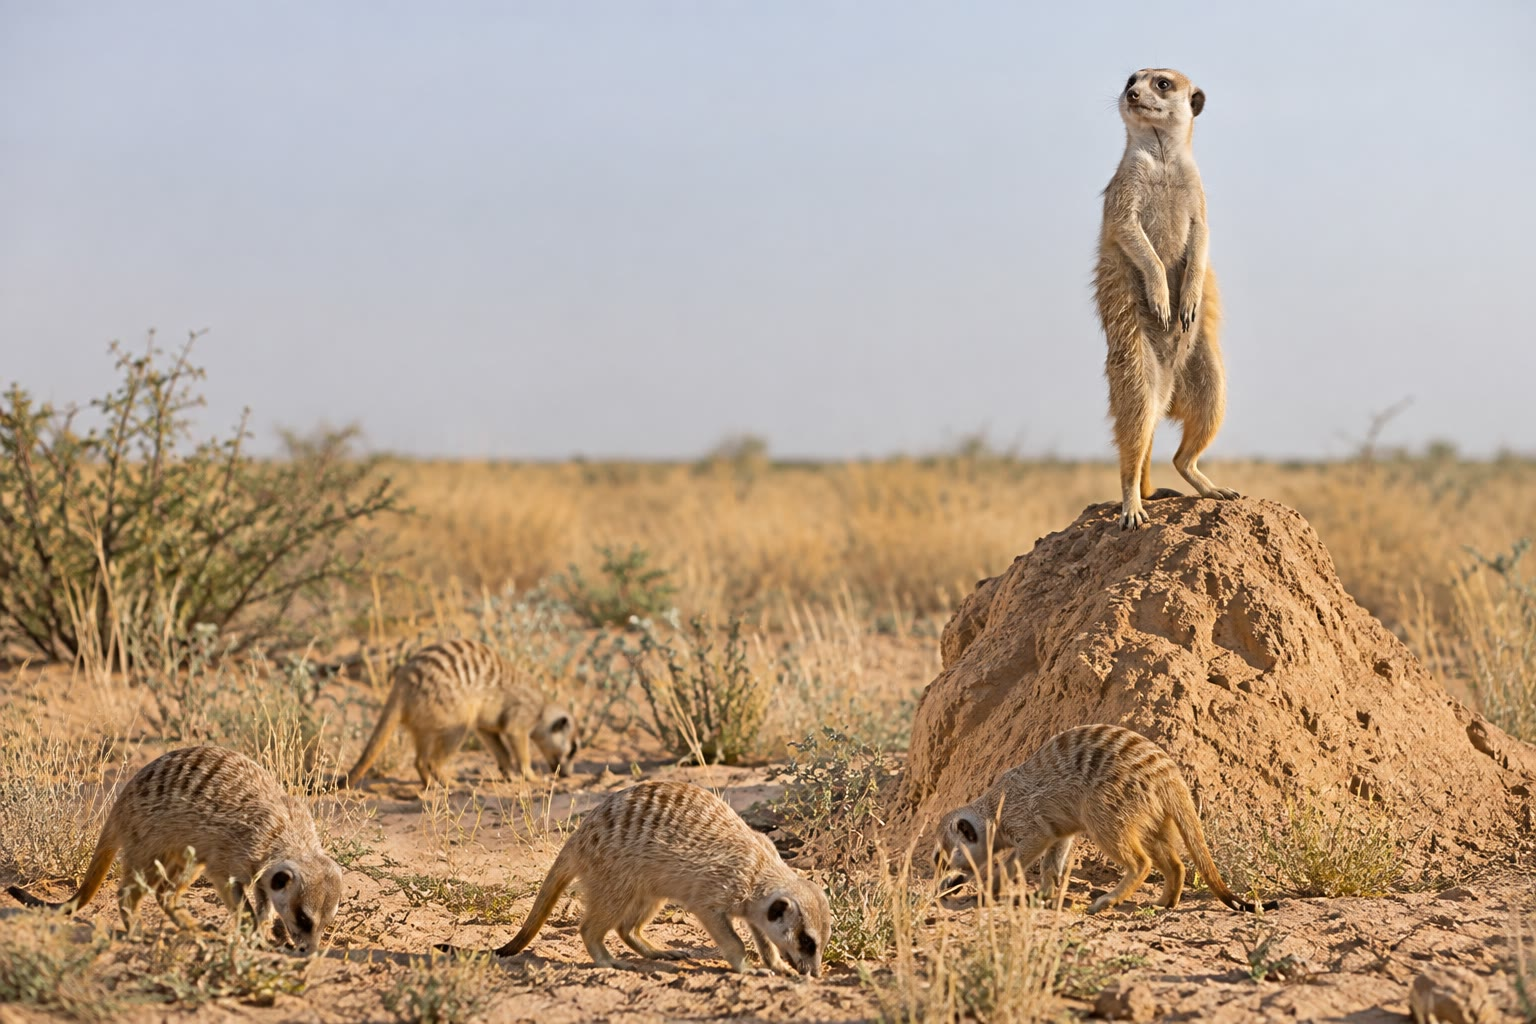
\includegraphics[width=0.46\linewidth]{images/book5/ai/b5-26-meerkat-sentinel.jpg}\hspace{0.04\linewidth}
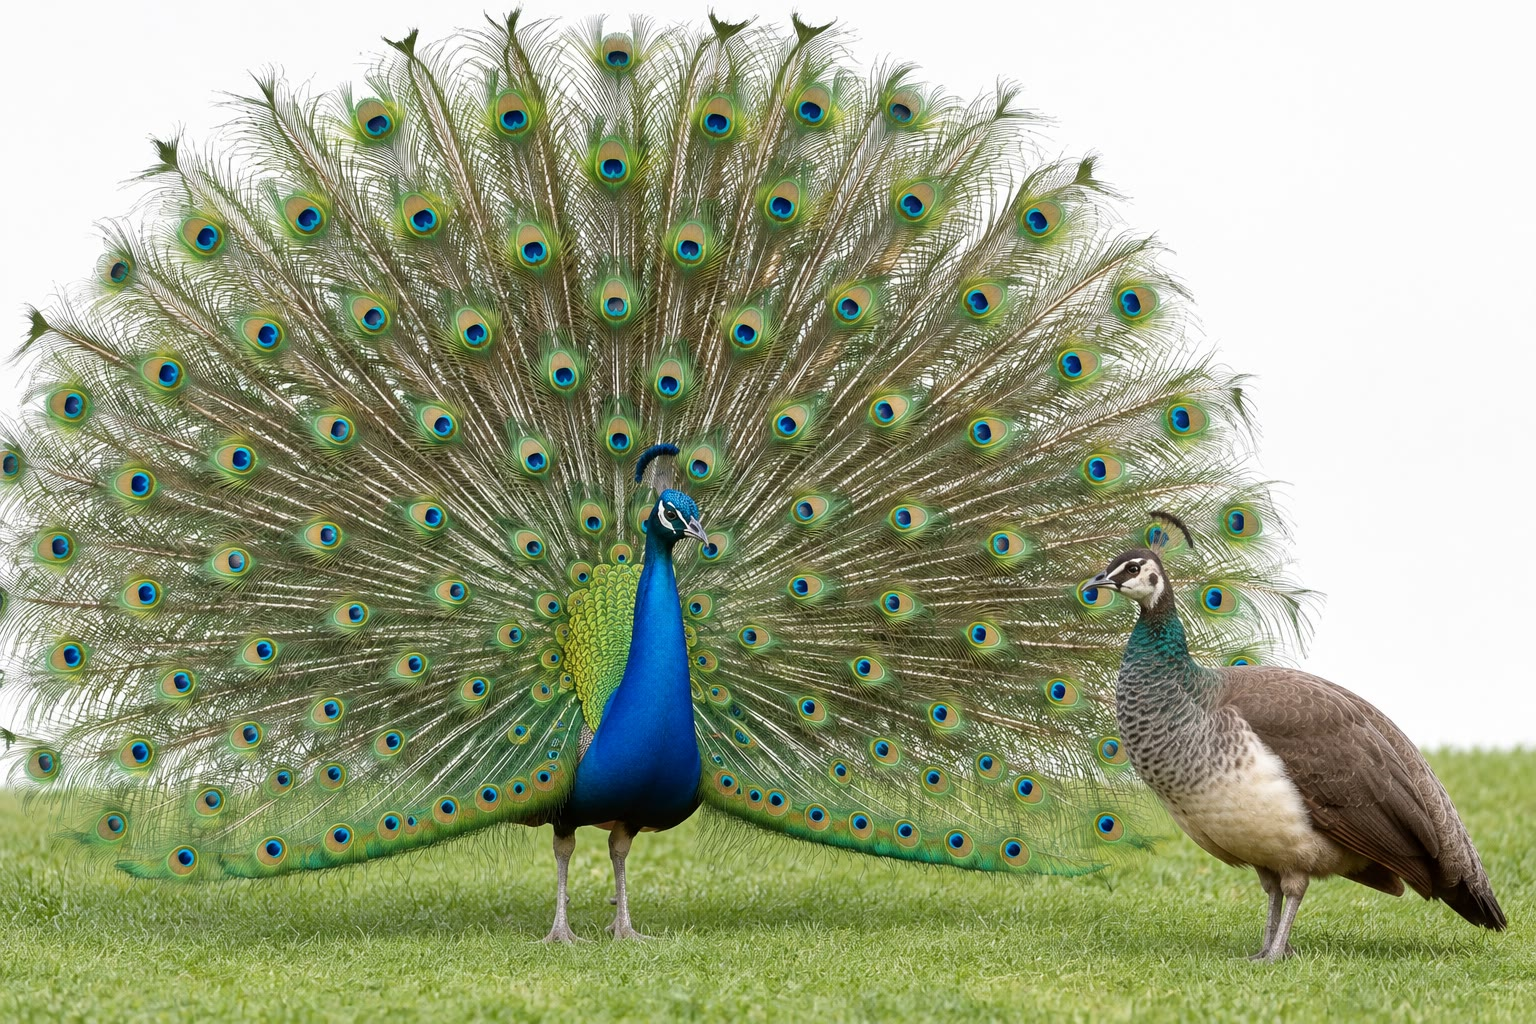
\includegraphics[width=0.46\linewidth]{images/book5/ai/b5-26-peacock-display.jpg}

{\small 左：一只猫鼬在觅食的亲属群体上方担任哨兵。
右：雄孔雀向雌孔雀展示，这种结构
使其携带者在食物和速度上付出代价，
换来的只是雌性的注意。}
\end{omfigure}

\section{配偶与信息}

\begin{definition}[性选择]\label{def:b3:behavioural-ecology:sexual-selection}
\index{性选择}\index{贝特曼梯度}\index{失控选择}\index{累赘原理}\index{优良基因}\index{性冲突}
达尔文的第二种机制：选择作用于赢得配偶而非生存的性状。
其根源在于异配生殖——雌性的繁殖
受其能产生并供养的卵子数限制，雄性的繁殖则受其能使之受精的雌性数限制，
因此在多数物种中，雄性的适合度随交配次数急剧上升，
而雌性的适合度几乎不随之上升（
\emph{贝特曼梯度}）；于是雄性争夺雌性，雌性
则在雄性中挑选。竞争带来角、鹿角、獠牙和较大的体型，
以及上一节中的争斗。择偶选择则带来装饰，
并有三种关于雌性为何偏好这些装饰的解释。费希尔的\emph{失控选择}：
雌性对稍长尾羽的偏好与长尾羽本身一同扩散，二者互相促进、彼此有利，
直到尾羽的生存代价
与其在交配中的收益相抵。扎哈维的\emph{累赘}：一种
只有健康雄性才负担得起生长的装饰，是诚实的
信号，表明其状况，正因为代价高昂——一只
尾屏饱满的雄孔雀已被证实寄生虫更少。\emph{优良基因}
和\emph{直接利益}：雌性获益的途径包括子代的遗传，
或通过雄性提供的领地和食物。
两性的利益并不一致，\emph{性冲突}——围绕
交配频率、谁来照顾幼体、以及前配偶精子的去向——
是同一物种内部进行的一场军备竞赛：
雄性果蝇的精液会缩短雌蝇的寿命，并提高其产卵量，
雌性则演化出抗性。
\end{definition}

\begin{proof}[证据]
安德森（1982）剪断并粘回了雄性长尾寡妇鸟的尾羽：
在肯尼亚，尾羽加长到自然长度两倍的雄鸟，
其领地吸引的新巢数量是尾羽缩短雄鸟的四倍，
而对照组尾羽同样被剪断、原样粘回的雄鸟，
则不受影响——雌性偏好的尾羽比任何雄鸟自然长出的都要长，
这是偏好已被选择到超出性状本身的标志。
彼得里（1994）发现，雌孔雀与尾屏上眼斑最多的雄孔雀交配，
且这些雄孔雀的幼鸟
在放归的林地中存活得更好——\omterm{def:b3:behavioural-ecology:sexual-selection}{优良基因}收益得到了测量。
贝特曼（1948）统计了携带标记突变的果蝇的交配次数和后代数，
发现了以他名字命名的梯度：
雄性的繁殖成功随交配次数线性上升，雌性的繁殖成功
在交配一次后便趋于平稳。
\end{proof}

\begin{proposition}[诚实信号]\label{prop:b3:behavioural-ecology:signals}
\index{通讯}\index{诚实信号}\index{摇摆舞}\index{指称性信号}
信号是一种改变接收者行为、并因此演化出来的行为，
只有当发送与响应对双方平均都有利时，它才是稳定的；
双方利益一致时，信号可以既廉价又精确：
觅食蜜蜂的\emph{\omterm{prop:b3:behavioural-ecology:signals}{摇摆舞}}（冯·弗里希，
20 世纪 40 年代）将食物源的方向编码为
摇摆路线与竖直方向的夹角——即食物源相对于太阳的角度——
而距离则以摇摆持续时间表示，约为每千米一秒，
招募来的蜜蜂会飞到距目标几十米以内；绿猴
针对豹、鹰
和蛇发出互不相同的警报声，听者对从隐藏扬声器播放的每种叫声都能做出恰当反应——
即\emph{指称性}信号。在利益相冲突的情况下，
信号必须代价高昂或无法伪造，才能保持诚实——
例如马鹿雄鹿的吼叫，其速率只有强壮的雄鹿才能维持；
蟾蜍鸣声的大小由其体型决定；上一段所述的装饰——
否则信号就会被利用：某属萤火虫模仿
另一属雌虫的闪光，以吃掉前来的雄虫；杜鹃的
雏鸟的乞食声压过了宿主自己的雏鸟。信号理论由此预测
信号的形式取决于双方的关系：
在利益一致的亲属与配偶之间，信号廉价而富于信息；
在对手之间，信号昂贵而程式化；捕食者与猎物之间则是一场军备竞赛。
\end{proposition}
\admitted

\begin{omfigure}
\begin{tikzpicture}[every node/.style={font=\scriptsize}, >=stealth]
  % field view
  \node[above] at (0,3.2) {野外};
  \draw[->, thick, gray] (0,0) -- (0,2.6) node[above, font=\tiny] {朝向太阳};
  \fill[omDef!60] (0,0) circle (0.12); \node[below, font=\tiny] at (0,-0.2) {蜂巢};
  \draw[->, very thick, omThm] (0,0) -- ({2.4*sin(40)},{2.4*cos(40)}); \node[right, font=\tiny, omThm] at ({2.4*sin(40)},{2.4*cos(40)}) {食物，\qty{1}{km}};
  \draw[omThm] (0,1.0) arc[start angle=90, end angle=50, radius=1.0]; \node[font=\tiny, omThm] at (0.55,1.25) {$40^{\circ}$};
  % comb view
  \begin{scope}[shift={(6.2,0)}]
    \node[above] at (0,3.2) {在竖直蜂脾上};
    \draw[very thick, gray!60] (-1.8,-0.4) rectangle (1.8,3.0);
    \draw[->, thick, gray] (0,0) -- (0,2.6) node[above, font=\tiny] {向上（= 太阳）};
    \draw[->, very thick, omThm] (0,0) -- ({1.6*sin(40)},{1.6*cos(40)}); \node[below, align=center, font=\tiny, omThm] at (0,-0.5) {摇摆路线：与竖直方向成 $40^{\circ}$；\\持续时间 $\approx \qty{1}{s}$ 每千米};
    \draw[omThm, dashed] ({1.6*sin(40)},{1.6*cos(40)}) .. controls (1.3,0.4) and (0.5,-0.3) .. (0,0);
    \draw[omThm, dashed] ({1.6*sin(40)},{1.6*cos(40)}) .. controls (-0.2,1.2) and (-0.6,0.3) .. (0,0);
    \draw[omThm] (0,0.8) arc[start angle=90, end angle=50, radius=0.8]; \node[font=\tiny, omThm] at (0.45,1.0) {$40^{\circ}$};
  \end{scope}
  \node[right, align=left] at (9.2,1.3) {一种符号编码：重力 \\代表太阳，时间 \\代表距离；招募来的蜜蜂 \\在数十米之内到达};
\end{tikzpicture}

{\small \omterm{prop:b3:behavioural-ecology:signals}{摇摆舞}。跑动路线与竖直方向的夹角即为
食物相对于太阳的角度；跑动长度即为距离。
如此廉价而又精确的信号之所以可能，
是因为舞者与其观众是利益相同的姐妹。}
\end{omfigure}

\begin{omfigure}
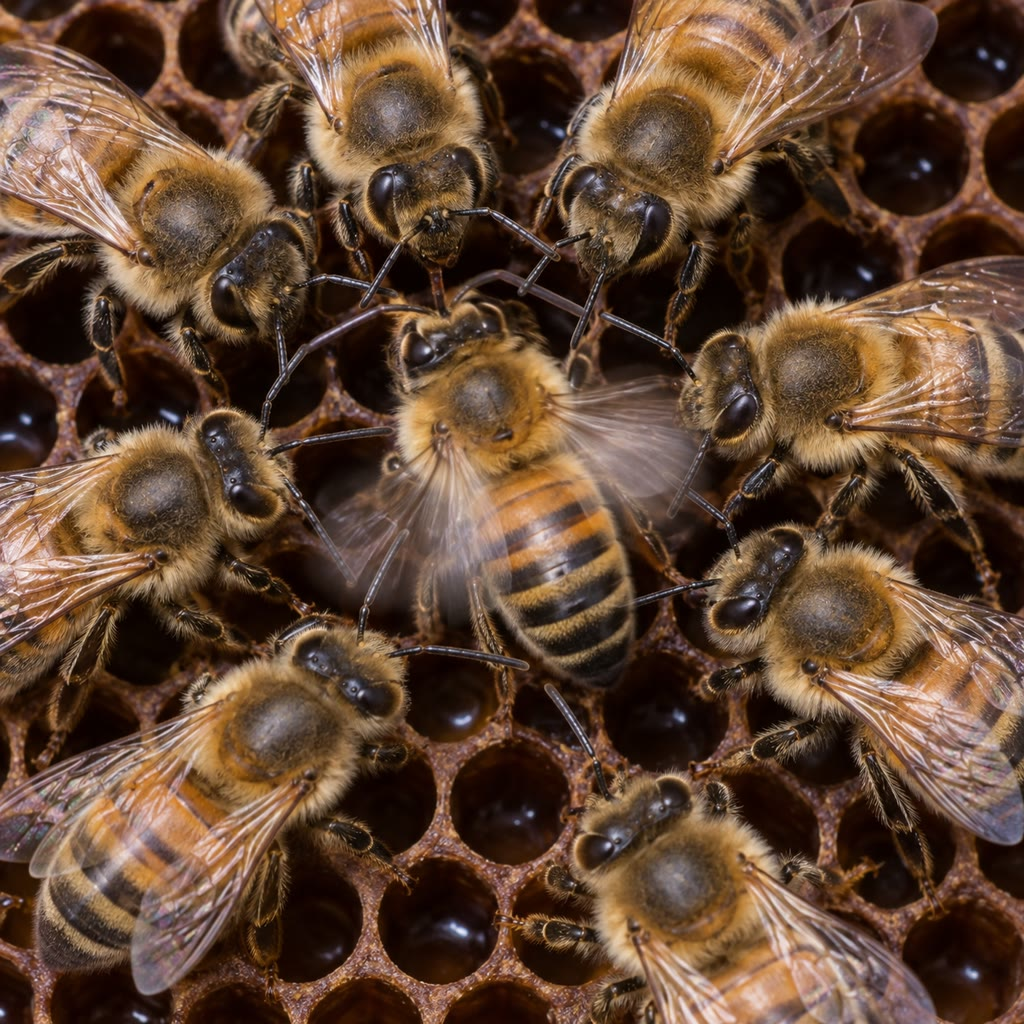
\includegraphics[width=0.4\linewidth]{images/book5/ai/b5-26-bee-dance.jpg}

{\small 一只觅食蜜蜂在蜂脾上跳舞，
周围环绕着读取其跑动角度与节奏的工蜂。}
\end{omfigure}

\begin{remark}[动物似乎在计算的原因]\label{rem:b3:behavioural-ecology:remark}
大山雀并不对 $g(t)/(\tau + t)$ 求导，猫鼬也不计算 $r$，
雌孔雀也从未听说过累赘。每种动物都遵循某些规则——
捕获速度变慢时离开，群体全为亲属时鸣叫，
偏好最鲜艳者——这些规则之所以被自然选择塑造，
是因为遵循它们的动物留下了更多后代；数学是我们的工具，
用来追问：为使这一点成立，规则必须达成什么目标，并预测动物在从未遇到过的情境中的行为。
当预测失败时——
山雀停留过久，哨兵的代价比预想的要小——
这种失败颇具\omterm{def:b3:bioinformatics:motif}{信息量}：收益尺度选错了，
某个约束被遗漏了，某位亲属被数错了。
这门学科是十年又十年地进行的，是野外笔记与一行代数式之间的对话，
而廷伯根提出的四个问题，
仍是两者共同的框架。
\end{remark}

\section{练习}

\begin{exercise}[$\star$]\label{exo:b3:behavioural-ecology:1}
叙述廷伯根提出的四个问题，
并针对\omterm{prop:b3:behavioural-ecology:signals}{摇摆舞}各用一句话作答。
\end{exercise}

\begin{exercise}[$\star$]\label{exo:b3:behavioural-ecology:2}
什么是\omterm{def:b3:behavioural-ecology:tinbergen}{固定动作模式}与\omterm{def:b3:behavioural-ecology:tinbergen}{信号刺激}？举两个例子，
并说明带有三道红色条带的“超常”木棒说明了什么。
\end{exercise}

\begin{exercise}[$\star$]\label{exo:b3:behavioural-ecology:3}
用文字叙述边际值定理说了什么，
以及当旅行时间加倍时，它对斑块利用作出了什么预测？
\end{exercise}

\begin{exercise}[$\star$]\label{exo:b3:behavioural-ecology:4}
给出 ESS 的定义。为什么纯鸽子种群不是 ESS，
而鹰–鸽混合会使所有个体付出代价？
\end{exercise}

\begin{exercise}[$\star\star$]\label{exo:b3:behavioural-ecology:5}
鹰–鸽博弈，$V = 6$，$C = 10$：求 $p^{*}$，
ESS 处每种策略的收益，以及全为鸽子的种群所得的收益，
对 $V = 12$，$C = 10$ 重复计算。
\end{exercise}

\begin{exercise}[$\star\star$]\label{exo:b3:behavioural-ecology:6}
一个获益函数 $g(t) = A(1 - \mathrm{e}^{-t/T_{0}})$，其中 $T_{0} =
\qty{2}{min}$。求 $t^{*}$，分别取 $\tau = 2$ 和 $\tau = 8$ 分钟（采用本章取值），
各斑块被消耗的比例，
以及长期速率 $R$（以每分钟占 $A$ 的比例计）。
\end{exercise}

\begin{exercise}[$\star\star$]\label{exo:b3:behavioural-ecology:7}
计算下列各对之间的 $r$：半同胞；祖父母与孙辈；
表兄弟姐妹；单倍二倍体工蜂与其兄弟；单倍二倍体蜂后与其儿子。
并说明后两种情况。
\end{exercise}

\begin{exercise}[$\star\star$]\label{exo:b3:behavioural-ecology:8}
报警鸣叫使鸣叫者承受 \qty{2}{\%} 的死亡机会，却使附近的 $n$ 只亲属
各自免于 \qty{1}{\%} 的死亡机会。若亲属为全同胞，对于哪些 $n$，哈密顿法则有利于鸣叫？
若为侄女呢？
若无亲缘关系呢？
\end{exercise}

\begin{exercise}[$\star\star$]\label{exo:b3:behavioural-ecology:9}
寡妇鸟的尾羽长 \qty{50}{cm}；延长至 \qty{75}{cm} 时，它吸引的巢数
是原来的两倍；缩短至 \qty{25}{cm} 时，则减半。若每增加
\qty{25}{cm} 尾长，存活率下降 \qty{20}{\%}，则哪一种尾长能使
交配次数与存活率的乘积最大？
自然尾长为何可能比它短？
\end{exercise}

\begin{exercise}[$\star\star\star$]\label{exo:b3:behavioural-ecology:10}
增加第三种策略——报复者。它的表现与鸽子相同，
但遭受攻击时会反击。写出它分别与鹰、鸽及自身对局时的收益
（对鹰时进行战斗：$(V - C)/2$；对鸽与对报复者时则平分：$V/2$）。
证明当 $V < C$ 时，报复者种群不会被鹰侵入，
并讨论鸽子能否
渗入该种群。
\end{exercise}

\begin{exercise}[$\star\star\star$]\label{exo:b3:behavioural-ecology:11}
在消耗战中，每位竞争者坚持的时间取自某一分布；
ESS 为指数分布，其均值为 $V/$（单位时间成本）。
试解释为何固定的坚持时间不能成为 ESS，
以及为何指数分布使仍在展示的对手，
其未来预期的坚持时长
与它已展示了多久无关。
\end{exercise}

\begin{exercise}[$\star\star\star$]\label{exo:b3:behavioural-ecology:12}
哈密顿关于单倍二倍性的论证预测：工蜂应更倾向于抚育姐妹（$r = 3/4$）
而非兄弟（$r = 1/4$），而蜂后对儿子与女儿的价值相同。
预测若由工蜂控制，蜂群应产生的繁殖个体性别比例；
若由蜂后控制，又应为多少？
试说明特里弗斯与黑尔发现了什么，以及
与多只雄性交配的蜂后会对该论证产生什么影响。
\end{exercise}

\section{问题：哨兵的算术}

\begin{problem}[{周末问题——以行为生态学的方式看猫鼬群体的一天：
边际值定理的斑块时间，
鹰鸽博弈的争斗及其演化稳定策略，哨兵值守与
单倍二倍体蜂巢的亲缘核算，以及装饰物的代价，
收束于斑块停留时间、鹰的频率与
哨兵的哈密顿阈值}]
\label{pb:b3:behavioural-ecology:1}
数据：觅食斑块，$g(t) = A(1 - \mathrm{e}^{-t/T_{0}})$，$T_{0}
= \qty{3}{min}$，$A = \qty{60}{kJ}$；斑块间的移动时间 $\tau =
\qty{3}{min}$（密集栖息地）或 \qty{12}{min}（稀疏栖息地）。争夺洞穴的
争斗：$V = 10$，$C = 30$（适合度单位）。哨兵：一小时的值守
使哨兵付出 $c = 0.03$ 个后代当量（觅食损失、
暴露风险）；它降低群体成员的被捕食风险，每位获得 $b = 0.01$
个后代当量；群体有 $n$ 名成员，平均
\omterm{thm:b3:behavioural-ecology:hamilton}{亲缘系数}为 $\bar r$。蜂巢：工蜂以同等付出抚育 $k$ 只姐妹或 $k$
只自己的女儿。装饰物：尾长 $L$ 给出
交配次数 $m(L) = L/20$，存活率 $s(L) = 1 - (L/100)^{2}$，$L$ 以厘米计。

\medskip
\noindent\textbf{第一部分——斑块。}
\begin{enumerate}
  \item 写出长期速率 $R(t)$ 与
        对此 $g$ 的边际值条件。
  \item 证明该条件可化为 $(\tau + t)/T_{0} = \mathrm{e}^{t/T_{0}}
        - 1$，并对 $\tau = T_{0}$ 求解（可试 $t = 1.15\,T_{0}$）。
  \item 对 $\tau = 4T_{0}$ 求解（可试 $t = 2.0\,T_{0}$）。
  \item 对每种情形，求以分钟计的停留时间、每个斑块的能量、
        被消耗的斑块比例，以及以 kJ/min 计的速率 $R$。
  \item 一条经验规则：“固定停留 \qty{5}{min} 后离开。”计算
        两种栖息地的 $R$，并与最优值相比。该规则
        是否足够好？
  \item 另一条规则：“若 \qty{20}{s} 内未捕获到猎物，
        便离开。解释这一放弃时间规则为何近似该定理，
        以及在各斑块丰富度不同的情形下，它
        会朝哪个方向失效。
\end{enumerate}

\medskip
\noindent\textbf{第二部分——争斗。}
\begin{enumerate}[resume]
  \item 写出收益矩阵，并求 $p^{*}$。
  \item 当 $p = 0.1$、$p = p^{*}$ 与 $p =
        0.6$ 时，鹰与鸽的收益各为多少？各情形下哪种策略会扩散？
  \item 求\omterm{prop:b3:behavioural-ecology:hawk-dove}{演化稳定策略}处的收益，并与全鸽种群的收益相比较。
        每次争斗中，种群因可能发生的
        争斗损失了多少？
  \item 干旱使 $V$ 升至 $40$（洞穴稀缺）。新的\omterm{prop:b3:behavioural-ecology:hawk-dove}{演化稳定策略}是什么？
        这对艰难年份的争斗有何预测？
  \item 资产者策略：“居留时为鹰，入侵时为鸽”，两种角色
        各占一半的时间。它与自身对局的收益为 $V/2$，无争斗；
        证明当 $V
        < C$ 时，鹰无法入侵资产者种群，并解释斑纹林蝶的情形。
  \item 用一句话解释为何该行为受频率依赖支配，
        而非最优化的支配。
\end{enumerate}

\medskip
\noindent\textbf{第三部分——亲缘。}
\begin{enumerate}[resume]
  \item 对哨兵应用哈密顿法则，以 $n\bar r$ 为条件。
        对于何种 $n\bar r$，值守才划算？
  \item 由 $n = 8$ 个全同胞组成的群体（$\bar r = 1/2$）：值守是否划算？
        由 8 只无亲缘关系的动物组成的群体呢？由 8 只半同胞组成的群体呢？
  \item 哨兵吃得很饱，因此其 $c$ 降至 $0.01$。阈值
        现在为多少？为何这预示哨兵多是
        吃得很饱的个体？
  \item 蜂巢：抚育 $k$ 只姐妹的\omterm{thm:b3:behavioural-ecology:hamilton}{广义适合度}，与抚育 $k$
        只女儿的\omterm{thm:b3:behavioural-ecology:hamilton}{广义适合度}相比。工蜂应偏好哪一种？比值为多少？
  \item 蜂后与三只雄性等量交配，工蜂与姐妹的
        平均\omterm{thm:b3:behavioural-ecology:hamilton}{亲缘系数}为多少？该偏好是否仍然成立？
  \item 解释为何哈密顿法则不要求行为者
        识别亲属，以及地松鼠实际可能采用
        何种经验规则。
\end{enumerate}

\medskip
\noindent\textbf{第四部分——装饰物。}
\begin{enumerate}[resume]
  \item 适合度 $W(L) = m(L)\,s(L)$。计算 $W$ 在 $L = 20$、$40$、$60$、
        $80$ 时的值。
  \item 以解析方法求 $L$，使 $W$ 取最大值，并求该处的 $W$。
  \item 存活代价加剧至 $s = 1 - (L/70)^{2}$（捕食者到来）。
        新的最优值为多少？朝哪个方向移动？为何这预示
        尾巴的演化会追随捕食压力？
  \item 安德森的实验把尾长加倍至 \qty{75}{cm}，并使巢数加倍。
        雌性对更长尾巴的偏好，这种“超过最优”
        是否符合\omterm{def:b3:behavioural-ecology:sexual-selection}{失控选择}的解释、累赘的解释，
        还是两者皆是？
  \item 为何廉价的装饰物不是\omterm{prop:b3:behavioural-ecology:signals}{诚实信号}，以及
        第~21~题中的代价如何使其成为\omterm{prop:b3:behavioural-ecology:signals}{诚实信号}？
  \item \omterm{def:b3:behavioural-ecology:sexual-selection}{贝特曼梯度}：每次额外交配，雄性获得 $0.8$ 个后代，
        雌性为 $0.1$ 个。试用一段话解释这种不对称
        如何同时产生第二部分的争斗与第四部分的
        装饰物。
  \item 总结：密集栖息地中的 $t^{*}$（第~4~题），$p^{*}$
        （第~7~题），以及哨兵的阈值 $n\bar r$
        （第~13~题）。
\end{enumerate}
\end{problem}
